\documentclass[class=book, crop=false, oneside, 12pt]{standalone}
\usepackage{standalone}
\usepackage{../../style}
\usepackage{../../style_tree}
\usepackage{../../style_automata}
\usepackage[normalem]{ulem}
\graphicspath{{./assets/images/}}

% arara: pdflatex: { synctex: yes, shell: yes }
% arara: latexmk: { clean: partial }
\begin{document}
\chapter[Parsing bottom-up: introduzione e SLR(1)]{Analisi sintattica: Introduzione al bottom-up parsing e parsing SLR(1)}
Iniziamo la trattazione del parsing di tipo \emph{bottom-up}: come suggerisce il nome stesso, consiste nel ricostruire le derivazioni di una parola in ordine inverso, partendo dall'ultima produzione usata per derivare la parola considerata, fino ad arrivare allo start symbol; a livello visivo, possiamo pensare che la nostra intenzione è di costruire un albero di derivazione partendo dalle foglie e arrivando alla radice. 

Prima di cominciare, un'avvertenza: questo argomento è molto complesso e la teoria sottesa è piuttosto criptica e pesante, per cui suggeriamo al lettore di dedicare molta attenzione agli esempi ed esercizi che presenteremo, perché a nostro avviso sono spesso fondamentali alla comprensione dello stesso impianto teorico su cui poggiano.

\section{Introduzione}
\subsection{Schema del processo}
\label{subsec:schema}
Durante questo e durante i prossimi capitoli andremo a conoscere diverse varianti del bottom-up parsing, che però condividono tutte lo stesso schema di operazioni da compiere. È uno schema diviso in quattro fasi, che andremo ad analizzare una ad una per ciascuna delle diverse varianti che incontreremo, per cui è bene conoscerlo subito e cercare di tenerlo a mente.
\begin{enumerate}
    \item All'inizio, altro non abbiamo se non una grammatica \(\G\) e una parola \(w\);
    \item la prima operazione sarà la costruzione di un automa caratteristico per la nostra \(\G\), che è semplicemente un automa a stati finiti simile ad altri che abbiamo già visto;
    \item una volta cche avremo l'automa, possiamo usarlo per calcolarne una tabella di parsing bottom-up;
    \item infine, utilizzando la tabella, lanceremo un algoritmo chiamato \texttt{shift/reduce} che, con l'ausilio della tabella appena calcolata, effettuerà il parsing vero e proprio della nostra parola \(w\) rispetto alla grammatica \(\G\).
\end{enumerate}
Consigliamo al lettore di tornare spesso a rivedere questo elenco numerato, perché la andremo a trattare ciascun passaggio in maniera piuttosto estesa e si rischia di perdere lo sguardo d'insieme del processo.

\subsection{Tipologie di parsing}
\paragraph{Le sigle}
Riprendiamo il discorso di quali sono le varianti di parsing bottom-up. In primis, è importante prendere familiarità coi loro criptici nomi; alcuni li abbiamo già intravisti nel parsing top-down, ora finalmente proponiamo un piccolo schema per imparare a dare del contesto a quelle sigle:
\begin{labeling}{LA}
    \item[S] sta letteralmente per "simple";  
    \item[L] l'input viene letto da sinitra;
    \item[R] verrà ricostruita una derivazione rightmost (analogamente per leftmost\footnote{Attenzione: questo schema può facilmente risultare fuorviante. Da quello che ci è stato spiegato sembra che, nel dare i nomi a queste classi di grammatiche, ci debbano essere almeno due lettere, la prima delle quali indica da quale direzione viene letto l'input, la seconda delle quali indica se la derivazione è leftmost o rightmost (quindi avremo LL(1): lettura da sinistra, derivazione leftmost, LR(1): lettura da sinistra, derivazione rightmost e via così); eventuali altre qualificazioni (come S o LA) sembrano essere inserite prima di quei due valori. \emph{La Quaglia non ha mai dato nessuna informazione su quanto questo schema sia rigido, e in realtà non ha nemmeno mai parlato di schema, per cui consigliamo di tenere gli occhi aperti}.});
    \item[1] leggeremo un simbolo alla volta;
    \item[LA] viene utilizzata una funzione \emph{lookahead};
\end{labeling}
Nella nostra trattazione parleremo soprattutto di SLR(1), LR(1) e LALR(1).

\paragraph{Classi di grammatiche}
Non tutte queste tecniche sono applicabili su tutte le grammatiche; infatti, la formulazione di ogni grammatica determina quale tecnica di parsing potrà essere applicata, tanto che solitamente si dice che è la grammatica stessa ad appartenere ad una determinata classe (quindi il lettore non si stupisca se fra poco inizieremo a parlare di grammatiche LR(1), SLR(1) et similia). In altre parole, noi diciamo che una grammatica \(\G\) appartiene a una certa classe di grammatiche, ad esempio LR(1), se siamo capaci di costruire una tabella di parsing di tipo LR(1) per \(\G\) (o di qualsiasi altro tipo stiamo considerando).
% \begin{itemize}
%     \item per qualsiasi grammatica \(\G\) considerata, andremo sempre a espandere il suo insieme \(\P\) in \(\P'\) aggiungendo la produzione \(S \to S'\), dove \(S'\) è un non-terminale \emph{fresh};
%     \item utilizzano i medesimi algoritmi \emph{shift} e \emph{reduce} (ne parleremo più avanti);
%     \item hanno sempre un automa a stati finiti, detto \emph{automa caratteristico}, il cui ruolo è di supervisionare il funzionamento dell'algoritmo di parsing.
% \end{itemize}
\paragraph{Differenze tra le classi}
Dipendentemente dalla classe di grammatica considerata, avremo automi caratteristici che rappresentano le informazioni in maniera più o meno dettagliata. Maggiore è il livello di dettaglio dell'informazione, più diventa grande e complesso l'automa caratteristico, ma anche più potente diventa il nostro parsing, inteso come numero di diverse grammatiche che può analizzare. Tra quelli presentati, il meccanismo più potente è LR(1), complementare del LL(1) che abbiamo visto nel parsing top-down; per questo motivo noi cercheremo sempre di costruire una tabella di parsing deterministico che rientri nei vincoli di LR(1). Se questo non sarà possibile andremo a scalare in complessità con LALR(1) e SRL(1).

\paragraph{Ampliamento di \(\P\)}
\label{par:p-newprod}
 Indipendentemente da quella che è la classe che consideriamo, quando siamo nell'ambito del parsing bottom-up andremo sempre ad ampliare l'insieme \(\P\) delle produzioni aggiungendo la produzione \(S \to S'\), dove \(S'\) è un non-terminale \emph{fresh} per la nostra grammatica \(\G\).

\section{Costruzione dell'automa}
Tuffiamoci subito nel primo passaggio, ossia la costruzione di un automa caratteristico a partire dalla grammatica data.

\subsection{Gli stati}
Andiamo per prima cosa a indagare quale forma avranno gli stati del nostro automa caratteristico. Gli stati sono degli insiemi di \emph{items}, dove gli items sono oggetti che avranno forma diversa, dipendentemente dalla tecnica di parsing utilizzata:
\begin{labeling}{LR(1)-items}
    \item[LR(0)-items] \(A \to \alpha \cdot \beta\)
    \item[LR(1)-items] [\(A \to \alpha \cdot \beta, L\)], dove \(L \subseteq T \cup \{\$\}\)\footnote{Ricordiamo che \(T\) è l'insieme dei terminali della grammatica considerata.}
\end{labeling}
Dalla definizione possiamo intuire cosa intendevamo quando prima abbiamo detto che gli LR(1)-items sono più ricchi dei loro corrispondenti LR(0), e ci permettono quindi di riconoscere grammatiche in modo più efficace: quell'insieme \(L\), come vedremo in seguito, contiene delle informazioni rispetto a quello che ci aspettiamo di leggere in futuro; nessuna informazine simile è presente negli LR(0)-items.

\paragraph{Esempio}
Andiamo a fare subito un esempio per aiutarci a capire di cosa stiamo parlando. Consideriamo la nostra fida grammatica:
\begin{equation}
    \label{eq:balanced}
    \G: S \to aSb \mid ab
\end{equation}
Come avevamo anticipato in \ref{par:p-newprod}, come prima cosa aggiungiamo alla grammatica una nuova produzione \(S' \to \cdot S\), e partiamo proprio da quest'ultima. Consideriamo il suo LR(0)-item \(S' \to \cdot S\): il significato intuitivo è che, se siamo all'inizio della procedura di parsing, siamo in una posizione in cui vogliamo conoscere quali sono le parole derivabili a partire da \(S\) (o, nel caso più generale, di qualsiasi cosa segua il marker \(\cdot\)), per cui è logico pensare che il nostro item \(S' \to \cdot S\) debba stare nello stato iniziale dell'automa, che chiamiamo \(P_0\).

Ma non sarà l'unico item a risiedere in \(P_0\).  Guardiamo bene \ref{eq:balanced}: analizzare la parola vuol dire aspettarsi qualcosa che derivi da \(aSb\) oppure \(ab\), per cui gli LR(0)-items di \(S\) saranno:
\begin{itemize}
    \item \(S \to \cdot aSb\);
    \item \(S \to \cdot ab\).
\end{itemize}
Questi verranno inseriti nel nostro \(P_0\), assieme all'item \(S' \to \cdot S\) che avevamo identificato prima. 

\subsection{Chiusura di un insieme di LR(0)-items}
Nel nostro esempio precedente abbiamo cercato di capire intuitivamente quali items è logico inserire negli stati, ma è chiaro che serve ben poca complessità per mettere fuori gioco il nostro intuito. Abbiamo bisogno di un procedimento formale per determinare quali items andranno inseriti nei vari stati, e per fare in questo ci viene in aiuto il concetto di chiusura di un insieme di LR(0)-items:

\begin{definition}
    Sia \(P\) un insieme di LR(0)-items; allora, \(closure_0(P)\) è il più piccolo insieme che soddisfa la seguente equazione:
    \begin{equation}
        closure_0(P) = P \cup \{B \to \cdot \gamma \; \mid \; A \to \alpha \cdot B \beta \in closure_0(P) \; \textrm{e} \; B \to \gamma \in P'\}
    \end{equation}
\end{definition}

La chiusura consiste sostanzialmente nell'aggiungere, per tutti quegli items che hanno un punto davanti ad un non-terminale, tutte le derivazioni possibili di quel non-terminale; questo va applicato ricorsivamente fino a che non sono presenti tutte le chiusure delle produizioni con un punto davanti ad un non-terminale. Più facile a farsi che a dirsi, credetemi, come del resto qualsiasi altro procedimento che vedremo in questo capitolo.

\subsubsection{Esempio di calcolo della chiusura}
Prendiamo ora ad esempio la seguente grammatica:
\begin{align*}
    E &\to E+T \mid T\\
    T &\to T*F \mid F\\
    F &\to (E) \mid id
\end{align*}
Come primo passo, consideriamo l'item \(E \to \cdot E\) e calcoliamone la chiusura \(closure_0(\{E' \to \cdot E\})\). Ecco il procedimento passo per passo:
\begin{enumerate}
    \item inizializziamo \(closure_0(\{E' \to \cdot E\})\) = \(\{E' \to \cdot E\}\); 
    \item andiamo a vedere se questo insieme contiene qualche marker davanti ad un non-terminale: effettivamente, c'è un marker prima di \(E\);
    \item aggiungiamo quindi le due produzioni di \(E\) alla chiusura \(\{E \to \cdot E+T\}\) e \(\{E \to \cdot T\}\);
    \item una volta aggiunte queste produzioni, vediamo ricorsivamente se si presentano altre situazioni con \(\cdot\) prima di un non-terminale;
    \item nel primo caso troviamo ancora \(\cdot E\), però abbiamo già analizzato la produzione \(E\), per cui possiamo passare oltre;
    \item nel secondo caso invece abbiamo \(\cdot T\) e non abbiamo ancora analizzato tutte le produzioni di \(T\), quindi andiamo ad aggiungere all'insieme le produzioni di \(T\);
    \item aggiungamo \(\{T \to \cdot T * F\}\) e \(\{T \to \cdot F\}\);
    \item ci troviamo di nuovo in un caso in cui abbiamo due nuove derivazioni con \(\cdot\) davanti
    a un non-terminale, ma \(\cdot T\) è già analizzato, per cui analizziamo solo \(\cdot F\);
    \item aggiungiamo le produzioni di \(F\): \(\{F \to \cdot (E)\}\) e \(\{F \to \cdot id \}\);
    \item siamo arrivati alla conclusione, e qui sotto è riportato l'insieme chiusura che abbiamo trovato:
\end{enumerate}
\begin{align*}
    E' &\to \cdot E \\
    E  &\to \cdot E+T \\
    E  &\to \cdot T \\
    T  &\to \cdot T * F \\
    T  &\to \cdot F \\
    F  &\to \cdot (E) \\
    F  &\to \cdot id
\end{align*}

Ora che ne abbiamo visto un'applicazione, formalizziamo questa proceduracon dello pseudocodice: solo per voi, l'algoritmo per il calcolo della chiusura:
% \begin{figure}[H]
%     \centering
%     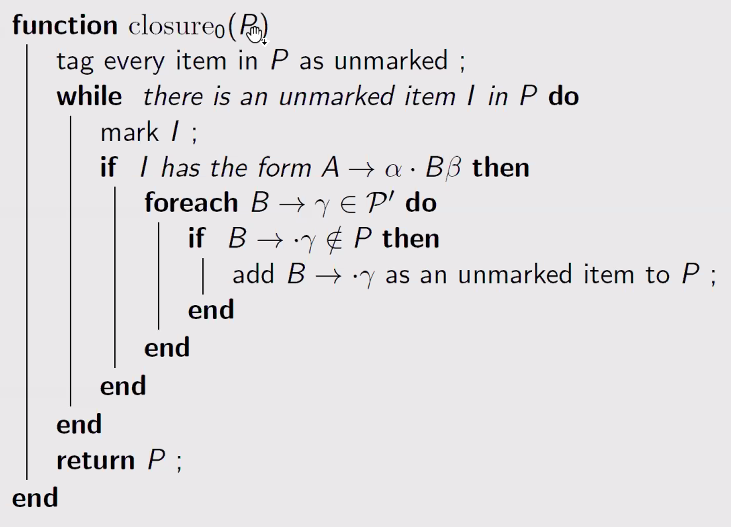
\includegraphics[width=.8\textwidth]{bottom-up-parsing_closure_algorithm.png}
%     \caption{Algoritmo per il calcolo di \(closure_0(P)\)}
% \end{figure}
\subimport{assets/pseudocode/}{lr0-closure.tex}

\subsection{Costruzione di un automa caratteristico per il parsing LR(0)}
Abbiamo visto cosa sono gli stati che compongono gli automi caratteristici; a questo punto siamo pronti per costruire il nostro primo automa caratteristico,  in questo caso per il parsing. La tecnica di costruzione è incrementale: andiamo a popolare un set di stati definendo mano a mano la funzione di transizione, fino a saturazione; il lettore si accorgerà che tale tecnica è poi utilizzata per costruire anche altri automi LR.

\subsubsection{Procedura}
\paragraph{Inizio}
In primis, definiamo il kernel dello stato iniziale come \(P_0 = \{S' \to \cdot S\}\), dove \(S'\) è un carattere inserito da noi, mentre \(S\) è lo start symbol della nostra grammatica.

\paragraph{Svolgimento}
Fino a che non esauriamo gli stati ancora da visitare andiamo a prenderli uno alla volta e li analizziamo nel segiente modo:
\begin{enumerate}
    \item calcoliamo il la chiusura del kernel dello stato, questo insieme rappresenta tutte le produzioni che si possono compiere da un certo stato per transitare verso altri stati;
    \item una volta calcolata la chiusura del kernel, le produzioni (gli item) che abbiamo già collezionato avranno forma \(A \to \alpha \cdot x \beta\), il che significa che nello stato in cui mi trovo, diciamo \(P\), ho già visto \(\alpha\) e posso fare una transizione tramite \(x\);
    \item esiste quindi una transizione da \(P\) a uno stato \(P'\) attraverso l'item \(A \to \alpha x \cdot \beta\); se \(x\) è un terminale, tale transizione rappresenta un'operazione di shift (come abbiamo visto nell'esercizio della sezione scorsa). Questo significa che avrò una transizione etichettata con \(x\) che mi porta da \(P\) a \(P'\);
    \item a questo punto genero il nuovo stato \(P'\) che contiene come kernel l'item \(A \to \alpha x \cdot \beta\), ricordando che poi andrò a includere tra gli item di \(P'\) anche gli item che appartengono a \(closure_0 (\{ A \to \alpha x \cdot \beta \})\), poiché se \(\beta\) è un non-terminale allora mi aspetto di poter trovare in \(P'\) anche tutto ciò che deriva da \(\beta\).
\end{enumerate}
C'è però una nota da aggiungere a questo procedimento: può accadere che quando generiamo un nuovo stato \(P'\) per transizione da uno stato \(P\) ci rendiamo conto che il kernel di questo stato corrisponde al kernel di un altro stato che abbiamo già vistisato, diciamo \(Q\); in questo caso invece che creare un nuovo stato \(P'\), quello che facciamo è collegare (tramite una \(x\)-transizione) \(P\) a \(Q\).

\subsubsection{Esempio di costruzione di automa LR(0)}
\label{subsubsec:esercizio_costruzione_automa_lr0}
Per consolidare la procedura sopra illustrata, andiamo subito a mettere le mani su un esempio di costruzione di un automa caratteristico per il parsing LR(0), in particolare per la seguente grammatica:
\begin{align*}
    S &\to aABe \\
    A &\to Abc \mid b \\
    B &\to d
\end{align*}

\paragraph{Inizio}
Partiamo creando lo stato iniziale, lo stato \(0\):
\begin{equation*}
    S' \to \cdot S
\end{equation*}
Ma c'è di più: nello stato iniziale va inserita anche la \(closure_0(\{ S' \to \cdot S \})\), quindi aggiungo le produzioni di \(S\): \(S \to \cdot aABe\). Dato che non sono presenti altre produzioni con marker prima di caratteri non-terminali, la chiusura dello stato \(0\) è completa.

\paragraph{Svolgimento}
A questo punto ci troviamo nello stato \(0\) ed abbiamo due produzioni, una con il marker prima di \(S\) ed una con il marker prima di \(a\), per cui dobbiamo aggiungere le seguenti transizioni:
\begin{enumerate}
    \item \(\tau (0, S) = 1\)\footnote{Come il lettore attento avrà già osservato, gli stati possono venire indicati con la notazione: \(\tau( \textrm{stato di provenienza}, \textrm{transizione di provenienza})\).}, ovvero una transizione che sta per "sono nello stato \(0\) e leggo \(S\) nell'input buffer";
    \item \(\tau (0, a) = 2\), ovvero una transizione che sta per "sono nello stato \(0\) e leggo \(a\) nell'input buffer".
\end{enumerate}
Questi stati però potrebbero essere già presenti! Non è questo il caso dato che sono i primi stati che troviamo, ma in seguito dovremmo ricordarci di tale controllo. \\

\begin{itemize}
    \item Partiamo con l'analizzare il nuovo stato \(\tau (0, S) =\) 1. \\
    Dobbiamo calcolare il \emph{kernel} dello stato, che si ottiene spostando il marker oltre al carattere che ci ha portati qui:
    \begin{equation*}
        S' \to S \cdot
    \end{equation*}
    Questo è quello che viene definito kernel dello stato; non presenta ulteriori transizioni possibili dato che il marker è arrivato in fondo, quindi passiamo ad analizzare un altro stato. 
    \item Andiamo ad analizzare lo \(\tau (0, a) =\) 2. \\
    Il kernel questa volta è:
    \begin{equation*}
        S \to a \cdot ABe
    \end{equation*}
    Dato che il kernel presenta almeno una produzione con un non-terminale alla destra del marker, dobbiamo aggiungere la chiusura del kernel a questo stato, ovvero:
    \begin{align*}
        A &\to \cdot Abc\\
        A &\to \cdot b
    \end{align*}
    Quindi gli item dello stato 2 sono:
    \begin{align*}
        S &\to a \cdot ABe\\
        A &\to \cdot Abc\\
        A &\to \cdot b
    \end{align*}
    Dallo stato 2 avremo quindi due possibili transizioni, una tramite \(A\) ed una tramite \(b\).
    \item Partiamo ad analizzare \(\tau (2, A) = 3\). \\
    Il kernel di questo stato è composto da due produzioni, dato che da \(2\) si può arrivare in \(3\) tramite due distinte produzioni:
    \begin{align*}
        S &\to aA \cdot Be \\
        A &\to A \cdot bc
    \end{align*}
    Per verificare se questo stato è già stato raggiunto, vado a verificare che non siano presenti stati con gli stessi item; in questo casp non ce ne sono, per cui lo stato \(3\) non è ancora stato effettivamente aggiunto e quindi lo tengo. Calcoliamo la chiusura dello stato, che ci porta ad aggiungere la seguente produzione:
    \begin{equation*}
        B \to \cdot d
    \end{equation*}
    Una volta calcolata la chiusura, mi segno i nuovi stati da visitare.
    \begin{itemize}
        \item \(\tau (3, B) = 5\)
        \item \(\tau (3, b) = 6\)
        \item \(\tau (3, d) = 7\)
    \end{itemize}
    \item Analizziamo ora lo stato \(\tau (2, b) = 4\). \\
    Questo stato ha come kernel:
    \begin{equation*}
        A \to b \cdot
    \end{equation*}
    e non presenta ulteriori possibili sviluppi, quindi passiamo oltre.
    \item Analizziamo lo stato \(\tau (3, B) = 5\). \\
    Il kernel in questo caso è:
    \begin{equation*}
        S \to aAB \cdot e
    \end{equation*}
    questo kernel è già chiuso (la sua chiusura, infatti, è un insieme vuoto) e ci offre come unica transizione possibile \(\tau (5, e) = 8\).
    \item Analizziamo lo stato \(\tau (3, B) = 6\). \\
    Il kernel in questo caso è:
    \begin{equation*}
        A \to Ab \cdot c
    \end{equation*}
    Anche questo kernel è già chiuso; ci offre la transizione allo stato \(\tau (6, c) = 9\).
    \item Analizziamo lo stato \(\tau (3, d) = 7\). \\
    Questo stato ha come kernel:
    \begin{equation*}
        B \to d \cdot 
    \end{equation*}
    Tale kernel è chiuso e non presnta transizioni uscenti.
    \item Non ci rimane che analizzare gli stati \(8\) e \(9\) che presentano rispettivamente i seguenti kernel:
    \begin{align*}
        S &\to aABe \cdot \\
        A &\to Abc \cdot
    \end{align*}
    entrambi i kernel non presentano ulteriori transizioni.
\end{itemize}

\paragraph{Conclusione}
In conclusione, l'automa caratteristico che otteniamo da questo procedimento può essere visualizzato in Fig.\ref{fig:charateristic-automata_cosntruction}
\begin{figure}[H]
    \centering
	\subimport{assets/figures/}{automa_LR_8-3-4.tex}
    \caption{Automa caratteristico LR(0) per la grammatica \ref{subsubsec:esercizio_costruzione_automa_lr0}}
    \label{fig:charateristic-automata_cosntruction}    
\end{figure}

Una volta terminata questa arzigogolata esercitazione possiamo dare un'occhiata all'algoritmo per la costruzione di un automa LR(0) in Alg.\ref{alg:char-automata}. \\
% \begin{figure}[H]
%     \centering
%     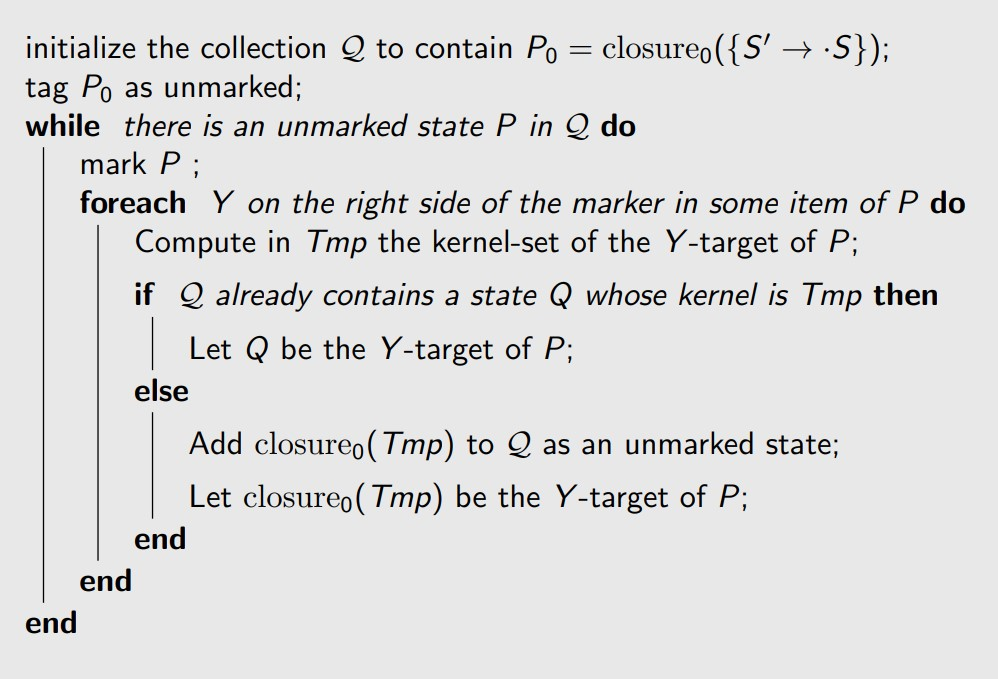
\includegraphics[width=.8\textwidth]{lr0-automata_construction_algorithm.jpg}
%     \caption{Algoritmo per la costruzione di un automa LR(0)}
%     \label{lr0-automata_construction_algorithm}    
% \end{figure}
\subimport{assets/pseudocode/}{char-automata.tex}

% Ma dove sono finite le etichette rosse che sull'automa dell'esercizio di shift/reduce ci segnalavano le mosse di reduce? Lo scopriremo nella prossima sezione.

\section{Costruzione di una tabella di parsing bottom-up}
\paragraph{Introduzione}
Ci stiamo avvicinando, fra poco parleremo dell'algoritmo shift/reduce, vero e proprio direttore d'orchestra del parsing. Questi compie delle mosse in base a cosa leggiamo su due pile ausiliarie (\(stSt\), pila degli stati, e \(symSt\), pila dei simboli), che sono valorizzate durante l'esecuzione a partire dalla parola considerata, e la decisione di quale mossa compiere è determinata dalla tabella di parsing della grammatica. Difatti, ora andremo a parlare di questa tabella.

\paragraph{Forma della tabella}
La tabella ha tante righe quanti gli stati dell'automa caratteristico, ed una colonna per ogni simbolo in \(V \cup \{ \$ \}\). La tabella dipende dall'automa caratteristico: automi diversi portano a tabelle diverse che portano a tipi di parsing diversi. 

\paragraph{Le riduzioni}
Le mosse di shift dipendono direttamente dalla funzione di transizione dell'automa, mentre le mosse di reduce sono più articolate: vanno effettuate solo quando raggiungiamo degli stati con etichette particolari, ed implicano che dobbiamo cancellare degli elementi dalla pila degli stati e dalla pila dei simboli, per poi inserire altri caratteri in quest'ultima pila. Inoltre, le mosse di reduce dipendono dal contenuto degli stati dell'automa: in un certo stato della tabella di parsing andiamo ad inserire una mossa di riduzione se la produzione \(A \to \beta\) è effettuata in uno stato contenente un reducing item per \(A \to \beta\). A questo punto però ci chiediamo: cosa sono i reducing item?
\begin{itemize}
    \item nel caso di LR(0)-items avranno forma \(A \to \beta \cdot\), e indicano che siamo arrivati alla fine della derivazione di \(\beta\), per cui il marker \(\cdot\) si trova in fondo alla derivazione;
    \item nel caso LR(1)-items avranno forma \(A \to \beta \cdot, \; \Delta\), e succede quando ho terminato l'analisi della produzione di \(\beta\),  ma con una condizione in più specificata da quel \(\Delta\).
\end{itemize}
Le riduzioni vengono applicate in base alla \emph{lookahead function} \(\mathcal{LA}\), la quale è definita per tutte le coppie \((P,\; A \to \beta)\) tali che \(P\) contiene un reducing item per \(A \to \beta\).

Da menzionare il fatto che la scelta dell'automa e della lookahead function per la costruzione della parsing table sono le caratteristiche che distinguono le varie tecniche di bottom-up parsing: la procedura di compilazione della tabella di parsing e l'esecuzione dell'algoritmo shift/reduce sono uguali per ogni classe considerata.

\subsection{Costruzione di una tabella di parsing generica}
Vediamo ora nello specifico come costruire una tabella di parsing. Abbiamo una tabella con delle entries di forma \(M[P, Y]\), dove \(P\) è uno stato e \(Y\) un simbolo del vocabolario \(V\), e dobbiamo riempire ciascuna di queste secondo le seguenti regole:
\begin{itemize}
    \item se \(Y\) è un terminale e \(\tau (P,Y) = Q\) inserisci la mossa \texttt{shift} Q;
    \item se \(P\) contiene un reducing item per \(A \to \beta\) e \(Y \in \mathcal{LA}(P, A \to \beta)\), inserisci la mossa \texttt{reduce} \(A \to \beta\) (notiamo che è in questa regola che emerge che le reduce dipendono dalla lookahead function);
    \item se \(P\) contiene l'accepting item e \(Y=\$\) inserisci \texttt{accept};
        \begin{itemize}
            \item nel caso degli automi LR(0) l'accepting item è \(\{S' \to S \cdot\}\);
            \item nel caso degli automi LR(1) l'accepting item è \(\{S' \to S \cdot, \; \Delta\}\);
        \end{itemize}
\item se \(Y\) è un terminale o \$ e nessuna delle condizioni precedenti è valida, inserisce \texttt{errore};
    \item se \(Y\) è un non-terminale e \(\tau (P, Y) = Q\) inserisci la mossa \texttt{goto} \(Q\).
\end{itemize}
L'informazione che è contenuta nella tabella di parsing in posizione \(M[P, Y]\) viene dunque utilizzata per stabilire che tipo di operazione effettuare durante il parsing, dipendentemente dallo stato \(P\) in cui ci troviamo e dal simbolo \(Y\)che leggiamo in cima all'input buffer, terminale o non-terminale che esso sia. Nonostante la grandezza della tabella dipenda dal tipo di algoritmo di parsing bottom-up che andiamo ad applicare e dalla funzione di lookahead (\(\mathcal{LA}\)), l'algoritmo che viene utilizzato per riempire la tabella rimane quello appena visto.

\subsection{Conflitti}
Visto che abbiamo già avuto modo di discutere di tabelle di parsing anche per il parsing di tipo top-down, risulta naturale metterle a confronto e chiedersi se, anche in questo caso, sia possibile ottenere dei \textbf{conflitti} (ovvero delle entries multiple defined). Questa situazione può verificarsi anche in questo caso in due differenti modalità: parleremo di
\begin{itemize}
    \item \textbf{s/r conflict} (o shift/reduce conflict) nel caso in cui almeno un entry della tabella di parsing contenga sia un'operazione di \texttt{shift} Q (data dal fatto che esiste una \(Y\)-transizione che va dallo stato \(P\), dove ci troviamo attualmente, allo stato \(Q\)), sia un'operazione di \texttt{reduce} \(A \rightarrow \beta\) (poiché \(P\) contiene un reducing item per \(A \rightarrow \beta\) e \(Y \in \mathcal{LA}(P, A \rightarrow \beta)\));
    \item \textbf{r/r conflict} (o reduce/reduce conflict) nel caso in cui almeno un entry della tabella di parsing contenga due operazioni di \texttt{reduce} per produzioni distinte.
\end{itemize}
La prossima domanda sorge spontanea: cosa accade quando abbiamo un conflitto? La conclusione che possiamo trarre è che, se stiamo eseguendo un parsing di un certo tipo per una grammatica \(\G\) e troviamo un conflitto mentre costruiamo la tabella, allora \(\G\) \emph{non} è una grammatica di quel particolare tipo; ad esempio, se troviamo un conflitto mentre costruiamo una tabella LR(1) per una grammatica \(\G\), allora \(\G\) non è LR(1).
% La prossima domanda sorge spontanea: cosa accade al parsing quando abbiamo un conflitto? Visto che nell'ambito del parsing bottom-up abbiamo già parlato di tre differenti classi di grammatiche, prendiamoci del tempo per analizzare ogni caso singolarmente: se troviamo almeno un conflitto in una tabella di parsing costruita per la grammatica \(\G\) per eseguire un parsing di tipo 
% \begin{itemize}
%     \item \(SLR(1)\), allora \(\G\) \textbf{non} è una grammatica \(SLR(1)\)
%     \item \(LALR(1)\), allora \(\G\) \textbf{non} è una grammatica \(LALR(1)\)
%     \item \(LR(1)\), allora \(\G\) \textbf{non} è una grammatica \(LR(1)\)
% \end{itemize}
\subsection{Costruzione di una tabella di Parsing SLR(1)}
Entriamo nel merito di come costruire una tabella di parsing SLR(1); questo è un parsing poco raffinato e le tabelle contengono meno informazioni, e questo è dovuto a due motivi:
\begin{enumerate}
    \item la loro costruzione ha come base di partenza un automa caratteristico con LR(0)-item;
    \item la funzione di lookahead è pari a \(\mathcal{LA}(P, A \rightarrow \beta) = follow(A)\) per ogni \(A \rightarrow \beta \cdot \in P\).
\end{enumerate}
Poiché repetita iuvant, ribadiamo che una grammatica \(\G\) è SLR(1) se e solo se la parsing table ottenuta secondo quelle prescrizioni non ha conflitti.

\subsubsection{Esempio di costruzione di tabella SLR(1)}
Proviamo a costruire la tabella di parsing \(SLR(1)\) per la seguente grammatica \(\G\):
\begin{align*}
    S &\rightarrow aABe \\
    A &\rightarrow Abc \mid b \\
    B &\rightarrow d
\end{align*}
Riconoscerete di certo questa grammatica, l'abbiamo già vista nella costruzione dell'automa caratteristico (si osservi Fig.\ref{fig:charateristic-automata-complete}). Tuttavia, il nostro obiettivo qui è costruire la tabella di parsing, e per farlo utilizzeremo i risultati ottenuti in precedenza: sappiamo infatti che lo stato \(1\) (anche indicato dal colore verde) è quello che contiene l'\textbf{Accepting Item}\footnote{Ovvero uno stato etichettato come \(Accept\) e che, se raggiunto, implicherà una conclusione con successo dell'algoritmo.}, mentre invece gli stati contenenti i \textbf{Reducing Item} (segnalati come stati finali) sono invece 4, 7, 8, 9. 
\begin{figure}[H]
    \centering
	\subimport{assets/figures/}{automa_bottom_up_8-3-4.tex}
    \caption{Automa Caratteristico per la parsing table bottom-up}
    \label{fig:charateristic-automata-complete}    
\end{figure}
In particolare, possiamo dire che i reducing item sono:
\begin{enumerate}
    \item \(\{A \rightarrow b \cdot\}\) per lo stato 4;
    \item \(\{B \rightarrow d \cdot\}\) per lo stato 7;
    \item \(\{S \rightarrow aABe \cdot\}\) per lo stato 8;
    \item \(\{A \rightarrow Abc \cdot\}\) per lo stato 9;
\end{enumerate}
Avendo a disposizione l'automa caratteristico e i dati sopra citati è dunque possibile costruire la tabella di parsing seguendo l'algoritmo per la costruzione di una tabella di parsing per il bottom-up parsing (ricordiamo all'utente distratto che siamo nell'ambito del parsing; parsing e chiudoing). Procediamo quindi in questo modo:
\begin{enumerate}
    \item creiamo una tabella con tante righe quanti sono gli stati nel nostro automa caratteristico (in questo caso da 0 a 9) e con tante colonne quanti sono i terminali (a cui va aggiunto il \$) e i non-terminali presenti all'interno della nostra grammatica (in questo caso abbiamo di conseguenza \emph{a b c d e \$ A B S});
    \item facendo riferimento all'automa caratteristico, se \(Y\) è un terminale e c'è una transizione \(\tau (P, Y) = Q\) (ovvero una transizione che va dallo stato \(P\) allo stato \(Q\) attraversando un arco con etichetta \(Y\)), allora inseriamo un'operazione di \texttt{shift} \(Q\) nella cella \(M[P, Y]\); ad esempio, nel nostro caso inseriremo \(M[0, a] = 2\);
    \item a questo punto è necessario calcolare i follow (e di conseguenza i first, Tab.\ref{tab:first-follow-SLR(1)parsing}), in quanto per poter inserire correttamente le operazioni di \texttt{reduce} abbiamo bisogno di avere queste informazioni per la funzione di lookahead (\(\mathcal{LA}\));
    \begin{table}[H]
        \centering
        \subimport{assets/tables/}{ptbu-follow.tex}
        \caption{LRS(1) Parsing Table - Calcolo Follow per Lookahead}
        \label{tab:first-follow-SLR(1)parsing}
    \end{table}
    \item una volta calcolati i followprocediamo così: per tutti gli stati \(P\) che contengono un redicing item \(A \to \beta\) (ad esempio, \(M[4, b] = A \rightarrow b\cdot\)), andiamo a inserire la mossa di reduce nella casella \(M[P, Y]\), dove \(Y\) è calcolato con la lookahead function come \(Y = LA(P, A \to \beta)\), nel nostro caso \(Y = follow(A)\); 
    \item inseriamo in posizione \(M[1, \$]\) l'operazione di \texttt{Accept}, in quanto 1 contiene un accepting item;
    \item a questo punto dovremmo valorizzare a \texttt{error} tutte quelle celle \(M[P, Y]\) dove \(Y\) è o \$ o un terminale che non ricade nei casi precedenti; tuttavia per una maggiore comprensione a livello visivo, nel nostro esempio queste celle verranno lasciate vuote;
    \item infine, inseriamo un'operazione del tipo \texttt{goto} \(Q\) per tutti quelle celle \(M[P, Y]\) dove \(Y\) è un non-terminale e per cui esiste una transizione \(\tau(P, Y) = Q\) (ad esempio \(M[0, S]\) = \texttt{goto} 1, come è anche osservabile dall'automa caratteristico).
\end{enumerate}
In Tab.\ref{tab:parsing-table-SLR(1)parsing} possiamo trovare il risultato finale dell'algoritmo. Ai fini di una corretta lettura della tabella, specifichiamo qui sotto alcune convenzioni che verranno impiegate per tenere il tutto conciso, come ad esempio:
\begin{itemize}
    \item l'operazione di \texttt{shift} \(Q\) verrà indicata con \(sQ\);
    \item l'operazione di \texttt{reduce} \(A \rightarrow \beta\) con \(rK\), dove \(K\) indica la \(K\)-esima riduzione; questa notazione è molto conveniente e abbassa il grado di entropia della tabella, ma in seguito forniremo anche una notazione estesa per queste riduzioni;
    \item \emph{Acc} indica l'accepting item;
    \item l'operazione di \texttt{Goto} \(Q\) verrà indicata semplicemente da Q.
\end{itemize}
\begin{table}[H]
    \centering
    \subimport{assets/tables/}{ptbu-complete.tex}
    \caption{Tabella di parsing SLR(1)}
    \label{tab:parsing-table-SLR(1)parsing}
\end{table}
Notiamo che sulla porzione sinistra della tabella troviamo i vari terminali (compreso \$) e, nelle varie entries, avremo mosse di shift, di reduce e delle celle valorizzate a \texttt{error}; a destra di questa, invece, troviamo i non terminali con le relative mosse di \texttt{goto}.
Specifichiamo quindi il significato dei vari \(rK\):
\begin{itemize}
    \item \(r1 = S \to aABe\)
    \item \(r2 = A \to Abc\)
    \item \(r3 = A \to b\)
    \item \(r4 = B \to d\)
\end{itemize}
Dal momento che \(\G\) dà origine a una nuova grammatica senza creare alcun conflitto, possiamo concludere che \(\G\) è SLR(1).

Prima di passare alla prossima sezione è necessario precisare che \emph{solamente} le celle vuote che hanno per colonna un terminale o \$ sarebbero valorizzate a \texttt{error}: infatti, le celle vuote che hanno per colonna un non-terminale rimangono semplicemente vuote, in quanto sono dei casi che non è possibile che si verifichino. 

\section{Algoritmo Shift/Reduce}
Infine, eccoci arrivati: possiamo finalmente presentare l'algoritmo di shift/reduce, che ricordiamo essere quell'algoritmo che usiamo per ottenere il parsing di una parola \(W\) data la tabella di parsing bottom-up di una certa grammatica \(\G\). Ricordiamo inoltre che l'algoritmo di s/r viene uisto indipendentemente dalla classe di parsing considerata.
\begin{itemize}
    \item \textbf{Input}: una stringa \(w\) e la tabella di parsing \(M\) per \(\G = (V, T, S, \P)\);
    \item \textbf{Output}: una derivazione di \(w\) in ordine inverso se \(w \in \mathcal{L}(\G)\) (per trovare i passi di derivazione che ci portano a \(w\) dovremo leggere tutte le reduce che abbiamo applicato in ordine inverso); otterremo invece \texttt{error} se \(w \notin \mathcal{L}(\G)\);
    \item \textbf{Inizializzazione}: Per l'algoritmo è necessario inserire all'interno dell'input buffer la stringa \(w\$\), e inoltre abbiamo bisogno di due strutture dati:
    \begin{itemize}
        \item \(stSt\) (state stack - pila degli stati), che viene inizializzata ponendo in cima lo stato \(P_0\) (ovvero prima chiusura dell'insieme di LR(0)-item);
        \item \(symSt\) (symbol stack - pila dei simboli).
    \end{itemize}
\end{itemize}

% \begin{figure}
%     \centering
%     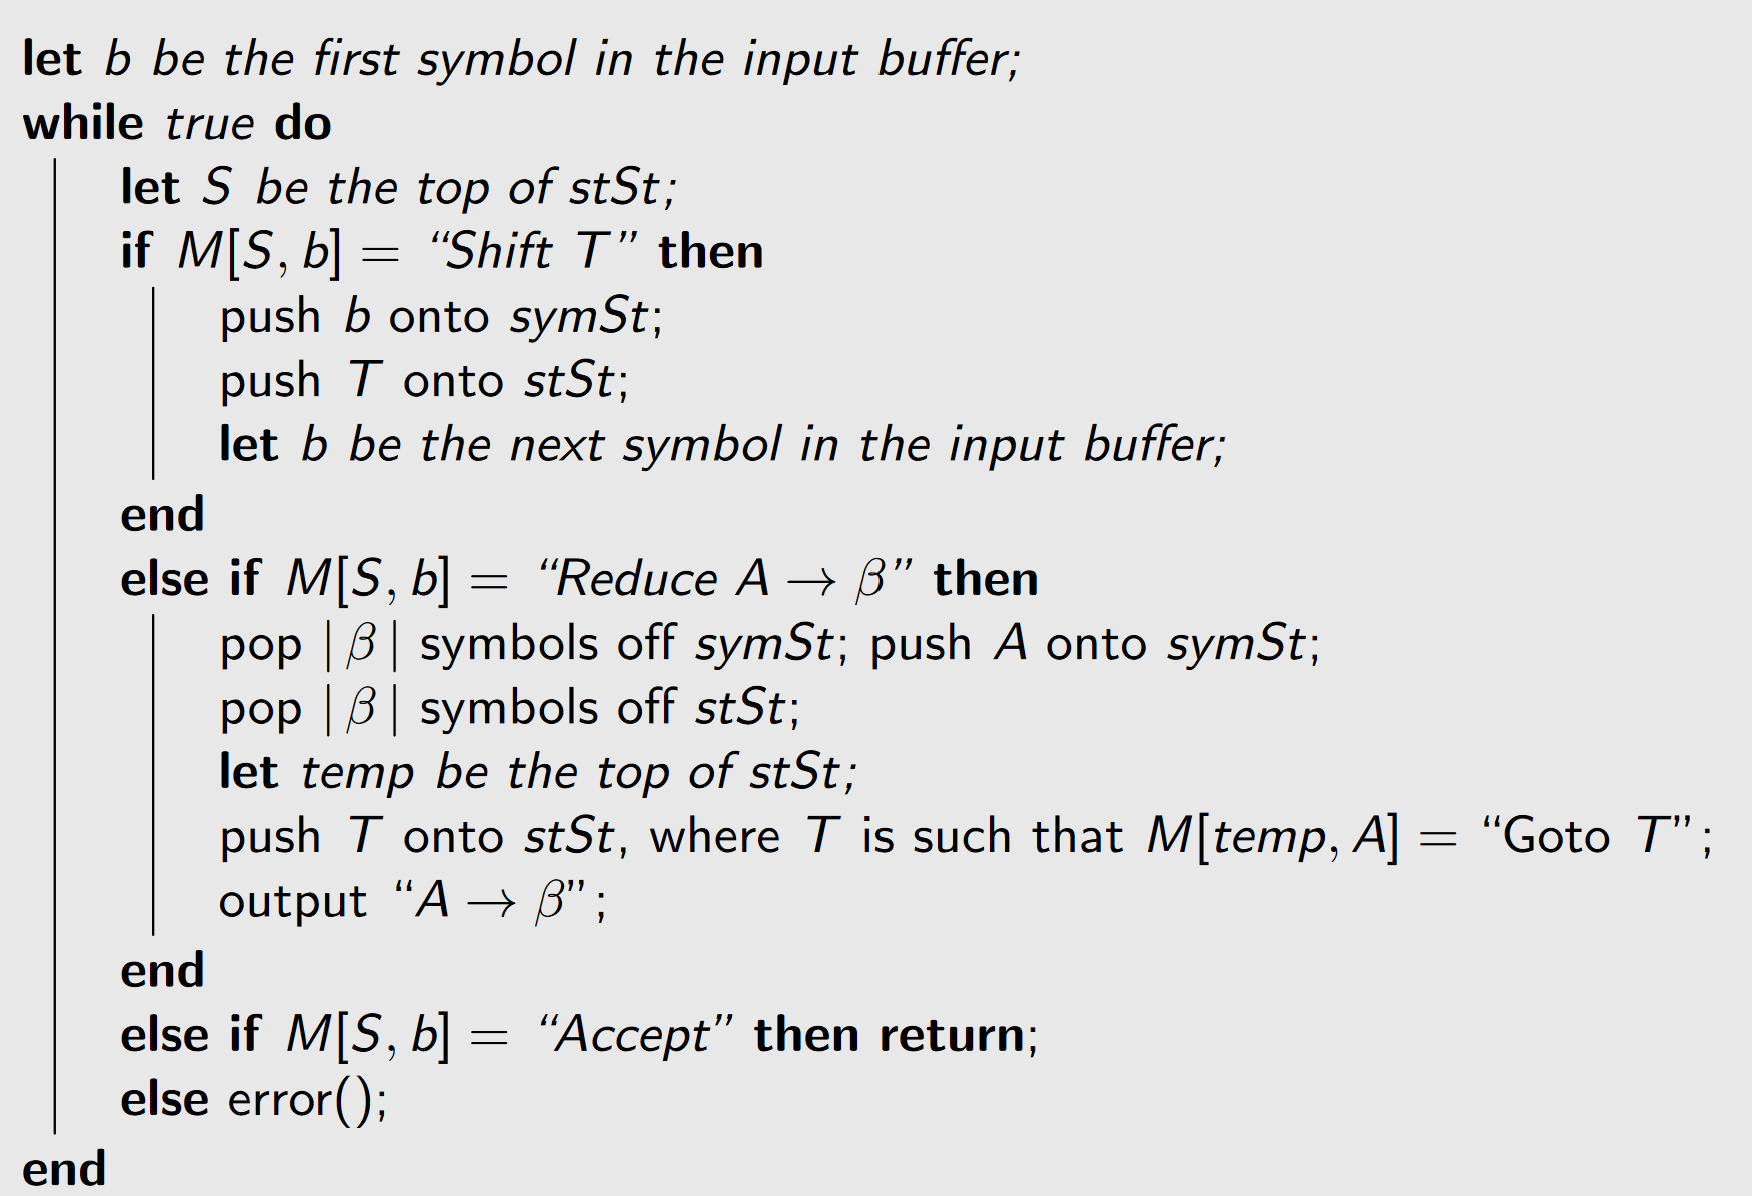
\includegraphics[width=.8\textwidth]{bottom-up-parsing-algorithm.png}
%     \caption{Algoritmo di parsing Bottom-Up}
%     \label{fig:bottom-up-parsing-algorithm}    
% \end{figure}
\subimport{assets/pseudocode/}{btmup-parsing.tex}
Andiamo subito a mettere in pratica questo algoritmo con un esempio.

\subsubsection{Esercizio shift/reduce 1}
Consideriamo questa parola:
\begin{equation*}
    w = abbcde
\end{equation*}
Andiamo a verificare se appartiene al linguaggio generato dalla grammatica:
\begin{align}
    \label{eq:grammar-ex-sh/re-1}
    \G: S &\to aABe \\
    A &\to Abc \nonumber \\ \notag
    A &\to b \nonumber \\ \notag
    B &\to d  \nonumber \notag
\end{align}
Ne abbiamo già calcolato la tabella di parsing bottom-up in Tab.\ref{tab:parsing-table-SLR(1)parsing}.

\paragraph{Svolgimento}
La configurazione iniziale è la seguente:
\begin{align*}
    w &= abbcde\$ \\
    stSt &= 0 \\
    symSt &= 
\end{align*}
Il primo carattere che leggiamo nel buffer è \(a\), per cui cerchiamo nella tabella del parsing il contenuto della casella [0,\(a\)]; scopriamo che contiene una mossa di shift verso lo stato 2, quindi andiamo ad inserire il nuovo stato di arrivo in \(stSt\) e il carattere letto in \(symSt\):
\begin{align*}
    w &= \underline{a}bbcde\$ \\
    stSt &= 0\;2\\
    symSt &= a
\end{align*}
Ci troviamo ora nello stato 2 e leggiamo il secondo carattere della parola che è \(b\), quindi controlliamo cosa contiene la casella [2,\(b\)] della tabella di parsing. Abbiamo un'altra mossa di shift che ci fa raggiungere lo stato 4 e leggere un altro carattere, e arriviamo quindi ad avere questa situazione:
\begin{align*}
    w &= \underline{ab}bcde\$ \\
    stSt &= 0\;2\;4\\
    symSt &= a\;b
\end{align*}
Ora siamo in 4 e leggiamo \(b\). La cella [4,\(b\)] ci suggerisce di compiere una mossa di reduce, nello specifico \(R: A \to b\); questo significa che compiremo due operazioni:
\begin{itemize}
    \item elimineremo tanti stati da \(stSt\) quanti gli elementi nel body della produzione (ovvero \(1\), dato che \(|b|\ = 1\));
    \item eliminiremo il body stesso da \(symSt\) e, al suo posto, inseriremo il driver della riduzione, in questo caso \(A\).
\end{itemize} 
Le nostre strutture saranno quindi valorizzate così: 
\begin{align*}
    w &= \underline{ab}bcde\$ \\
    stSt &= 0\;2\;\xout{4}\\
    symSt &= a\;A
\end{align*}
Ora però dobbiamo sostituire lo stato 4 con lo stato che è presente nella tabella in posizione [2,\(A\)], ovvero lo stato 3; la situazione si ristabilisce quindi così:
\begin{align*}
    w &= \underline{ab}bcde\$ \\
    stSt &= 0\;2\;3\\
    symSt &= a\;A
\end{align*}
Dobbiamo ancora consumare la \(b\) (le mosse di reduce non consumano i caratteri), quindi ora ci troviamo nella casella [3, \(b\)],e questa ci suggerisce la mossa shift 6; vediamo cosa succede:
\begin{align*}
    w &= \underline{abb}cde\$ \\
    stSt &= 0\;2\;3\;6\\
    symSt &= a\;A\;b
\end{align*}
A questo punto la casella da guardare diventa [6,\(c\)], che ci dice shift 9, ob-la-di, ob-la-da:
\begin{align*}
    w &= \underline{abbc}de\$ \\
    stSt &= 0\;2\;3\;6\;9\\
    symSt &= a\;A\;b\;c
\end{align*}
Plot-twist! proprio mentre ci siamo abituati alla tranquillità delle mosse di shift la casella [9,\(d\)] ci lascia sbigottiti con una mossa di reduce \(R: A \to Abc\), costringendoci ad eliminare ben 3 stati da \(stSt\) e 3 caratteri da \(symSt\) e sostituendoli con una sprezzante \(A\):
\begin{align*}
    w &= \underline{abbc}de\$ \\
    stSt &= 0\;2\;\xout{3\;6\;9}\\
    symSt &= a\;\xout{A\;b\;c}A
\end{align*}
A questo punto siamo costretti a guardare in [2,\(A\)] per capire in quale stato siamo stati sballottati dal \texttt{goto}, e scopriamo che siamo malaugaratamente tornati nello stato 3:
\begin{align*}
    w &= \underline{abbc}de\$ \\
    stSt &= 0\;2\;3\\
    symSt &= a\;A
\end{align*}
Bene, riprendiamo con la lettura: eravamo rimasti a \(d\), per cui ora controlliamo [3,\(d\)], che ci suggerisce shift 7:
\begin{align*}
    w &= \underline{abbcd}e\$ \\
    stSt &= 0\;2\;3\;7\\
    symSt &= a\;A\;d
\end{align*}
Stato 7, il prossimo carattere nel buffer è \(e\) e la casella [7,\(e\)] presenta questa riduzione \(R: B\to d\); ormai la prassi ci è nota (e prestate attenzione al fatto che in [3, \(B\)] troviamo \texttt{goto} 5):
\begin{align*}
    w &= \underline{abbcd}e\$ \\
    stSt &= 0\;2\;3\;\xout{7}\;5\\
    symSt &= a\;A\;\xout{d}\;B
\end{align*}
Dobbiamo ancora leggere la \(e\) e ci troviamo ora nello stato 5, e [5,\(e\)] ci dice shift 8:
\begin{align*}
    w &= \underline{abbcde}\$ \\
    stSt &= 0\;2\;3\;5\;8\\
    symSt &= a\;A\;\;B\;e
\end{align*}
Con 8 come stato e \$ come carattere in lettura ci assicuriamo una bella reduce in forma di \(R: S \to aABe\), che ci fa arrivare a questa situazione (ricordiamoci del \texttt{goto}):
\begin{align*}
    w &= \underline{abbcde}\$ \\
    stSt &= 0\;1\\
    symSt &= 
\end{align*}
Il prossimo passo è descritto dalla casella [1,\$], che ci dice Accept; questo significa che abbiamo terminato la verifica e possiamo dire, con somma pace interiore, che \(w \in \L(\G)\).

Non abbiamo solo trovato una soluzione al quesito iniziale, ma abbiamo anche ricavato i passi di derivazione che ci portano ad ottenere la parola \(w\) stessa; questi. infatti, consistono nelle riduzioni che abbiamo incontrato nel nostro cammino elencate in senso contrario:
\begin{align*}
    S &\to aABe &(aABe)\\
    B &\to d &(aAde)\\
    A &\to Abc &(aAbcde)\\
    A &\to b &(abbcde)
\end{align*}

\subsubsection{Il parsing dell'oca}
Ai più attenti non sarà di certo sfuggito che questa stregoneria del parsing è stata fortemente ispirata dal gioco dell'oca. Pensiamoci: è come se, nel nostro parsing dell'oca, l'obiettivo del gioco fosse quello di raggiungere una casella nascosta "dietro al via"\footnote{Abbiamo fiducia nel fatto che i nostri venticinque lettori stiano al gioco e riescano a intuire il senso di quest'espressione un po' criptica; la prima volta che l'ho letta pure a me suonava molto simile a quella storiella che i terrapiattisti tanto amano sui presunti racconti dei presunti diari di Richard Byrd, in cui l'ammiraglio affermerebbe di essersi spinto centinaia di miglia "oltre il Polo Sud". "Dietro al via", "Oltre il Polo", figata, no? \textasciitilde pips}. Abbiamo tre tipi di caselle:
\begin{itemize}
    \item le caselle di shift ci fanno avanzare di una casella;
    \item le caselle di reduce ci fanno indietrggiare di qualche casella;
    \item le celle error ci fanno perdere il gioco.
\end{itemize}
Purtroppo il tabellone di gioco non è un semplice percorso rettilineo, ma è una cosa più brutta che assomiglia un po' a un grafo. In compenso, nella nostra versione il percorso della pedina è \emph{deterministico}: non c'è un lancio dei dadi, c'è una sorta di mappa da seguire, che altro non è se non la parola \(w\) che vogliamo analizzare. E infatti l'obiettivo del nostro gioco è quello di prendere una mappa (ovvero una parola), seguirla e verificare se riusciamo ad arrivare alla casella finale con delle opportune reduce (perché ripetiamolo, la casella finale si trova "dietro all via!"). E quindi, cosa succede quando arriviamo alla casella finale? Succede che abbiamo vinto, perché vuol dire che la mappa che abbiamo seguito è valida, ovvero che la parola \(w\) considerata appartiene alla grammatica \(\G\) che ha generato il tabellone di gioco (ovvero il linguaggio); inoltre, possiamo anche capire esattamente come \(w\) deriva da \(\G\), seguendo il nostro percorso al contrario e annotandoci le mosse di reduce effettuate. Questo era tutto, siamo finalmente riusciti a dispiegare il nostro parsing una volta per tutte! \textasciitilde sam

Ottimo, adesso che abbiamo messo le cose in chiaro possiamo passare a un secondo esercizio, tanto più complesso quanto più completo e divertente del primo.

\subsubsection{Esercizio shift/reduce 2}
La consegna è di costruire la parsing table SLR(1) per la seguente, ormai ben nota, grammatica:
\begin{equation}
    \label{eq:ex2-sh/re-grammar}
    E \to E+E \mid E*E \mid id
\end{equation} 
Per costruire una parsing table abbiamo prima di tutto bisogno di ricavare l'automa a stati finiti determinato da tale grammatica.
\paragraph{Costruzione dell'automa}
\begin{enumerate}
    \item Inizializziamo lo stato 0; il suo kernel è 
    \begin{equation*}
        E' \to \cdot E
    \end{equation*}
    Di questo kernel devo calcolare la chiusura:
    \begin{align*}
        E &\to \cdot E+E \\
        E &\to \cdot E*E \\
        E &\to \cdot id
    \end{align*}
    Essendo questi gli item per lo stato 0, posso identificare due possibili transizioni (e quindi due possibili nunovi stati): \(\tau(0,E)=1 \textrm{ e } \tau(0,id)=2\).
    \item Analizziamo ora lo stato 2; il suo kernel è 
    \begin{equation*}
        E \to id \cdot    
    \end{equation*}
    Non serve calcolare la chiusura di questo item; inoltre, tale item non comporta transizioni uscenti dallo stato 2, per cui terminiamo qui l'analisi.
    \item Passiamo al vaglio lo stato 1, il cui kernel è popolato da questi item:
    \begin{align*}
        E' &\to E \cdot\\
        E  &\to E \cdot +E \\
        E  &\to E \cdot *E
    \end{align*}
    Tutti gli elementi del kernel sono già chiusi, e ci offrono queste transizioni: \(\tau(1,+)=3 \textrm{ e } \tau(1,*)=4\). Fatto ciò, abbiamo concluso l'analisi dello stato 1.
    \item Passiamo allo stato 3, il cui kernel risulta
    \begin{equation*}
        E \to E+ \cdot E
    \end{equation*}
    Tale kernel presenta però la possibilità di chiusura, per cui aggiungiamo la chiusura agli item dello stato 3, che risultano essere:
    \begin{align*}
        E &\to E+ \cdot E \\
        E &\to\ \cdot E+E \\
        E &\to\ \cdot E*E \\
        E &\to\ \cdot id
    \end{align*}
    Quindi, da qui posso transizionare tramite \(E\) e tramite \(id\). La transizione per \(E\) mi porta in \(\tau(3,E)=5\), la transizione per \(id\) invece è particolare: mi porterebbe in uno stato che ha come kernel \(E \to id.\), ma quello è lo stesso kernel dello stato 2! Quindi \(\tau(3,id)=2\).
    \item Analizziamo lo stato 4, che ha per kernel
    \begin{equation*}
        E \to E*.E 
    \end{equation*}
    Si può effettuare la chiusura, quindi gli item dello stato 4 sono:
    \begin{align*}
        E &\to E*.E \\ 
        E &\to .E+E \\
        E &\to .E*E \\
        E &\to .id
    \end{align*}
    Esistono due possibili transizioni uscenti dallo stato 4: una per \(E\), che genera lo stato \(\tau(4,E)=6\), e una per \(id\), che come per il caso precedente non genera un nuovo stato ma va a finire nello stato 2.
    \item Quando analizzo lo stato 5, trovo che il kernel è
    \begin{align*}
        E &\to E+E. \\
        E &\to E.+E \\
        E &\to E.*E
    \end{align*}
    Questo non necessita di chiusura, e ci fornisce due possibili transizioni:
    \begin{itemize}
        \item quella per \(+\), che però ci porta in uno stato con kernel \({E \to E.+E}\), ovvero nello stato 3, che abbiamo già analizzato;
        \item quella per \(*\), che però ci porta in uno stato con kernel \({E \to E.*E}\), ovvero nello stato 4, che abbiamo già analizzato.
    \end{itemize}
    \item Allo stesso modo, per lo stato 6 il kernel è
    \begin{align*}
        E &\to E*E. \\
        E &\to E.+E \\
        E &\to E.*E
    \end{align*}
    e nemmeno questo necessita di chiusura, e perdipiù, attraverso le due transizioni per \(+\) e per \(*\), ci porta esattamente negli stati 3 e 4.
\end{enumerate}
Una volta terminata l'analisi degli stati e dei relativi item ci preoccupiamo di trovare quali stati contengono l'accepting item e quali stati contengono i reducing item:
\begin{itemize}
    \item l'accepting item nel metodo SLR(1) è l'item \(S' \to S.\) (ovvero \(E' \to E.\)), che nel nostro caso è contenuto nello stato 1;
    \item i reducing item sono quelli con il marker \(\cdot\) al termine di una produzione, nel nostro caso sono \(E \to id \cdot\) (stato 2), \(E \to E+E \cdot\) (stato 5) e \(E \to E*E \cdot\) (stato 6).
\end{itemize}

Per concludere la parte di costruzione dell'automa caratteristico per la nostra grammatica in Eq.\ref{eq:ex2-sh/re-grammar}, inseriamo in Fig.\ref{ex2-sh/re-automata} il disegno di tale sgorbio (scherzo, è carino, sembra un razzetto).
\begin{figure}[H]
    \center
	\subimport{assets/figures/}{automa_caract_8-4.tex}
    \caption{Automa caratteristico per la grammatica \ref{eq:ex2-sh/re-grammar}}
    \label{fig:ex2-sh/re-automata}
\end{figure}

\subsection{Gestione dei conflitti}
Quindi, partendo dalla grammatica Eq.\ref{eq:ex2-sh/re-grammar} siamo riusciti a ricavarne e l'automa caratteristico SLR(1) in Fig.\ref{fig:ex2-sh/re-automata} e i reducing items, che ricordiamo essere:
\begin{align*}
    2: E &\to id & 5: E &\to E + E \cdot & 6: E &\to E * E \cdot
\end{align*}
Tutto questo è fantastico, ma purtroppo c'è un grosso elefante nella nostra stanza. L'intrinseca ambiguità di Eq.\ref{eq:ex2-sh/re-grammar} ha un effetto collaterale piuttosto sgradevole: la sua tabella di parsing SLR(1) avrà dei conflitti, come possiamo ben vedere in Tab.\ref{tab:ex2-sh/re-table}.
\begin{figure}[H]
    \center
    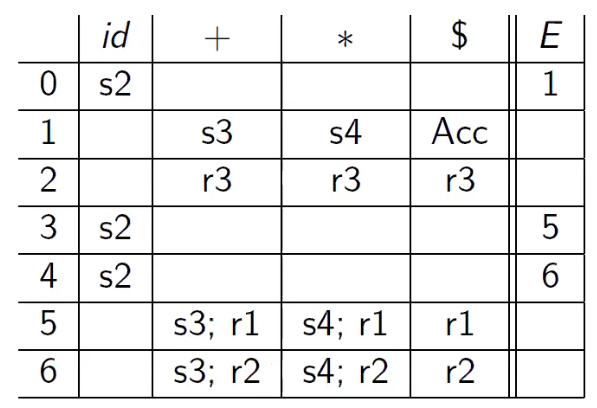
\includegraphics[width=.6\textwidth]{ex2-sh_re-table.png}
    \caption{tabella di parsing SLR(1) per la grammatica \ref{eq:ex2-sh/re-grammar}}
    % \label{tab:ex2-sh/re-table}
\end{figure}
\begin{table}[H]
    \centering
    \subimport{assets/tables/}{ex2-sh/re-table.tex}
    \caption{tabella di parsing SLR(1) per la grammatica \ref{eq:ex2-sh/re-grammar}}
    \label{tab:ex2-sh/re-table}
\end{table}
\noindent Quindi, se vogliamo perseguire la nostra ricerca di un parsing deterministico (e lo vogliamo), toccherà rimboccarsi le maniche e andare a capire come possiamo risolvere questi conflitti, non diversamente da quanto già avevamo fatto nel parsing top-down con le entries multiple defined.

I nostri conflitti sono localizzati solo in quattro situzioni, ossiamo quando ci troviamo in uno tra gli stati 5 o 6 e, contemporaneamente, troviamo in lettura un simbolo tra \(+\) o \(\ast\).
% \begin{figure}[H]
%     \centering
%     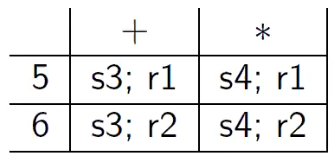
\includegraphics[width=.6\textwidth]{ex2-sh_re-table_conf.png}
%     \caption{Dettaglio di Tab.\ref{tab:ex2-sh/re-grammar_conf}}
%     % \label{tab:ex2-sh/re-table_conf}
% \end{figure}
\begin{table}[H]
    \centering
    \subimport{assets/tables/}{ex2-sh/re-table_conf.tex}
    \caption{Dettaglio di Tab.\ref{tab:ex2-sh/re-grammar_conf}}
    \label{tab:ex2-sh/re-table_conf}
\end{table}

\paragraph{La situazione}
Proviamo a capire bene qual è il punto di tutta questa situazione. Se il nostro parser si trova nello stato 5, questo vuol dire che, in testa alla nostra pila dei simboli \(symSt\), avremo necessariamente \(E + E\); possiamo vederlo facilmente, è sufficiente buttare un occhio al nostro automa caratteristico (Fig.\ref{fig:ex2-sh/re-automata}) per renderci conto che lo stato 5 è raggiungibile solo dallo stato \(3\), il quale a sua volta può essere raggiunto o dalla sequenza di stati \((0, 1)\), \((4, 6)\) o \((3, 5)\), in tutti questi casi sulla testa di \(symSt\) si troverà \(E + E\). Il discorso è del tutto analogo se passiamo allo stato 6, dove avremo la testa di \(symSt\) popolata di \(E * E\), poiché 6 è raggiungibile tramite \(\dots \to 0 \to 1 \to 4 \to 6\), \(\dots \to 4 \to 6 \to 4 \to 6\) oppure \(\dots \to 3 \to 5 \to 4 \to 6\).

È chiaro che abbiamo dei conflitti quando siamo nella situazione in cui due simboli legati da un operatore sono stati già letti (\(E + E\) o \(E * E\)) e, subito dopo, leggiamo un terzo simbolo. Questo è dovuto proprio al fatto che la grammatica, nella sua ambiguità, non riesce a esprimere opportunamente né associatività, né precedenza per i due operatori.

E insomma, qual è il segreto per risolvere questi dannati conflitti? Quello che faremo (almeno in questo caso) è, per ogni cella in cui abbiamo un conflitto, scegliere manualmente quale mossa mantenere\footnote{Qualcuno potrebbe a ragione pensare che, in questo modo stiamo barando, e a dirla tutta avrebbe ragione; ma nel reame dei compilatori è meglio tenere la conscienza sporca e fare del parsing efficace  rispetto a conservare l'integrità ma fare del parsing leeeeento.}. Questa scelta pare essere in mano nostra, e nel nostro specifico esempio faremo sì che il parser finisca per conformarsi a quelle che sono le comuni regole di precedenza e associatività per \(+\) e \(*\). 

\paragraph{L'utilità dei parse trees}
Possiamo aiutarci se pensiamo ai parse tree della nostra grammatica: gli alberi, infatti, per loro stessa costruzione, veicolano informazioni sull'annidamento dei loro elementi in maniera molto efficace, e l'annidamento può tranquillamente avere una corrispondenza diretta con la parentesizzazione. Di fatto assumendo, come facciamo noi, che i sottoalberi vengano risolti prima degli alberi padri, stabiliamo delle regole di precedenza del tutto simili a quelle che si possono ottenere con una parentesizzazione.

Nello specifico, noi siamo interessati a esprimire l'associatività sinistra degli operatori \(+\) e \(*\), nonché la precedenza di \(*\) rispetto a \(+\). Diciamolo in maniera ancora più pragmatica: se guardiamo gli esempi in Fig.\ref{fig:ex2-sh_re-ptree}, vogliamo sempre avere l'albero Fig.\ref{fig:ex2-sh_re-ptree_1} al posto di Fig.\ref{fig:ex2-sh_re-ptree_2} quando stiamo valutando una stessa espressione (\(E + E + E\), ad esempio), e vogliamo che la precedenza tra i due operatori sia tale da generare sempre parse tree come Fig.\ref{fig:ex2-sh_re-ptree_3} e Fig.\ref{fig:ex2-sh_re-ptree_4}: \(E*E\) è più "in basso", ergo verrà eseguita prima, ergo avrà precedenza su \(E+E\).
\begin{figure}[H]
    \begin{minipage}[b]{.4\textwidth}
        \centering
        \subimport{assets/figures/}{parse_tree_left_associative_a.tex}
        \subcaption{Parse tree left-associativo}
        \label{fig:ex2-sh_re-ptree_1}
    \end{minipage}
    \hfill
    \begin{minipage}[b]{.4\textwidth}
        \centering
        \subimport{assets/figures/}{parse_tree_left_associative_b.tex}
        \subcaption{Parse tree right-associativo}
        \label{fig:ex2-sh_re-ptree_2}
    \end{minipage}
    
    \begin{minipage}[b]{.4\textwidth}
        \centering
        \subimport{assets/figures/}{parse_tree_left_associative_c.tex}
        \subcaption{Parse tree per \(E * E + E\)}
        \label{fig:ex2-sh_re-ptree_3}
    \end{minipage}
    \hfill
    \begin{minipage}[b]{.4\textwidth}
        \centering
        \subimport{assets/figures/}{parse_tree_left_associative_d.tex}
        \subcaption{Parse tree per \(E + E * E\)}
        \label{fig:ex2-sh_re-ptree_4}
    \end{minipage}
    \caption{}
    \label{fig:ex2-sh_re-ptree}
\end{figure}
In questa interpretazione possiamo vedere le mosse di reduce come una parentesizzazione, perché stiamo assegnando un padre a un determinato sottoalbero del tipo \(E + E\) o \(E * E\)\footnote{QUesta frase è importantissima e invitiamo il lettore a spenderci alcuni minuti, perché afferrarne appieno il significato implica di aver ottenuto una buona comprensione del parsing bottom -up.}.

\paragraph{Risoluzione dei conflitti}
A questo punto possiamo andare ad analizzare i quattro conflitti che abbiamo trovato e, per ciascuna cella, scegliere la mossa che rende il parsing conforme alle regole che abbiamo stabilito. Tenendo a mente Tab.\ref{tab:ex2-sh/re-table_conf}, rimbocchiamoci le maniche.
\begin{itemize}
    \item \(M[5, +]\): questa è la situazione in cui la testa di \(symSt\) è popolata di \(E + E\) e in lettura troviamo un altro \(+\); gli operatori sono left-associativi, per cui vogliamo parentesizzare la testa del nostro \(symSt\) e solo dopo leggere il nuovo simbolo; ergo, la mossa che scegliamo e inseriamo in \(M[5, +]\) è \(r1\).
    \item \(M[6, *]\): vediamo subito questa cella perché presenta una situazione del tutto analoga a quella appena vista;  la testa di \(symSt\) è popolata di \(E * E\) e questa volta l'operatore coinvolto è \(\ast\), che al pari di \(+\) è left-associativo, di conseguenza anche qui scegliamo la reduce \(r2\) per dare precedenza alla parentesizzazione;
    \item \(M[5, *]\): torniamo adesso a parlare dello stato 5; la testa di \(symSt\) è popolata come prima, ma questa volta il lettura troviamo un simbolo \(\ast\). Questo cambia le carte in tavola, perché noi vogliamo che l'operatore \(\ast\) abbia precedenza più alta di \(+\); per ottenere questo, scegliamo la mossa di shift \(s4\), il che significa che rimandiamo la parentesizzazione della testa di \(symSt\) e proseguiamo nella lettura.
    \item \(M[6, +]\): qui abbiamo trovato \(E * E\) nella testa di \(symSt\) e ci sta arrivando un \(+\) in lettura, e ormai l'idea dovrebbe essere chiara: coerentemente con le regole di precedenza (\(\ast \prec +\)), vogliamo che la testa di \(symSt\) sia parentesizzata prima di proseguire con la lettura di \(+\), per cui qui teniamo la reduce \(r2\).
\end{itemize}
% \begin{figure}[H]
%     \centering
%     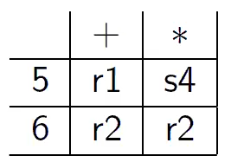
\includegraphics[width=.6\textwidth]{ex2-sh_re-table_conf_solved.png}
%     \caption{Soluzione dei conflitti di Tab.\ref{tab:ex2-sh/re-grammar_conf}}
%     \label{tab:ex2-sh/re-table_conf_solved}
% \end{figure}
\begin{figure}[H]
    \centering
    \subimport{assets/tables/}{ex2-sh/re-table_conf_solved.tex}
    \caption{Soluzione dei conflitti di Tab.\ref{tab:ex2-sh/re-grammar_conf}}
    \label{tab:ex2-sh/re-table_conf_solved}
\end{figure}
Fatto! Dopo tutto questo processo abbiamo ottenuto una tabella di parsing senza conflitti, ovvero senza entries multiple defined. Strategie di questo tipo sono abbastanza standard per le grammatiche degli operatori (non solo aritmetici, si pensi alle precedenze dell'algebra booleana); all'atto pratico, chi scrive le grammatiche (che ha studiato LFC e ha capito questi argomenti) si preoccuperà anche di predisporre delle direttive per il parser, sicché quest'ultimo abbia informazioni su quali scelte compiere in caso di conflitti.

\subsubsection{Un altro approccio: riscrivere la grammatica}
Naturalmente, tutto questo è reso necessario dal fatto che la grammatica \(\G\) in Eq.\ref{eq:ex2-sh/re-grammar} è ambigua; se avessimo semplicemente scritto un'altra grammatica \(\G'\) non ambigua, tale che \(\L(\G) = \L(\G')\), saremmo riusciti a ottenere una tabella di parsing senza conflitti da risolvere. Dovessimo percorrere questa strada, sia chiaro che è estremamente importante che la nuova grammatica esprima correttamente le regole di precedenza e associatività che vogliamo. Guardiamo ad esempio:
\begin{align}
    \label{eq:ex2-sh/re-grammar_v2}
    \G': E &\to E + T \mid T \\
    T &\to T * id \mid id \notag
\end{align}
L'ordine con cui ho inserito le produzioni non è causale: abbiamo posizionato \(*\) in un livello di produzione inferiore a \(+\) perché, dal momento che la derivazione è rightmost e andiamo ad attraversare l'albero dal basso verso la radice (bottom-up, no?), ci assicuriamo in questo modo di parentesizzare prima tutte le occorrenze di \(\ast\); non avremmo avuto questa garanzia se avessimo inserito produzioni come, ad esempio, \(E \to T + E\). 

Inoltre, se ad esempio avessimo scritto \(T \to id * T\), avremmo perso la left-associatività per l'operatore \(\ast\) (ma lo stesso sarebbe successo anche per \(+\)). Il modo migliore per convincersi di queste cose (nonché il nostro suggerimento per il lettore), è quello di provare da sé a cambiare la grammatica, provare a tracciare dei parse tree e vedere cosa succede, un po'come abbiamo fatto noi qui sotto in Fig.\ref{fig:ex2-sh_re-altgrm-ptree}.
\begin{figure}[H]
    \begin{minipage}[b]{.4\textwidth}
        \centering
        \subimport{assets/figures/}{parse_tree_left_associative_a_V2.tex}
        \subcaption{\(T \to T * id\), left-associativa (versione corretta)}
        \label{fig:ex2-sh_re-altgrm-ptree_1}
    \end{minipage}
    \hfill
    \begin{minipage}[b]{.4\textwidth}
        \centering
        \subimport{assets/figures/}{parse_tree_left_associative_b_V2.tex}
        \subcaption{Se invece scriviamo \(T \to id * T\) perdiamo la left-associatività}
        \label{fig:ex2-sh_re-altgrm-ptree_2}
    \end{minipage}
    \caption{Esempio di come possiamo alterare Eq.\ref{eq:ex2-sh/re-grammar_v2} e vedere i cambiamenti direttamente dalla struttura dei parse trees}
    \label{fig:ex2-sh_re-altgrm-ptree}
\end{figure}

È bene far notare, inoltre, che questo procedimento ci ha portato ad aggiungere il non-terminale \(T\) alla grammatica. Certo, un non-terminale in più non ha tutto questo grande impatto sull'efficienza degli algoritmi, ma in altre situazioni la scrittura di una grammatica non ambigua che generi un linguaggio equivalente (a quello della grammatica ambigua di partenza, ndr) può rivelarsi davvero complicata e costosa; per questo motivo, spesso si preferisce semplicemente tenere le grammatiche ambigue e gestire i conflitti manuealmente, tramite direttive per il parser: il prezzo da pagare per usare una grammatica non ambigua equivalente sarebbe troppo alto.

\subsubsection{Esercizio sulla risoluzione dei conflitti}
Sia data la seguente grammatica:
\begin{align}
    \label{eq:ex3-slr1-grammarr}
    \G: S &\to aAd \mid bBd \mid aBe \mid bAe \\
    A &\to c \nonumber \\ \notag
    B &\to c \notag
\end{align}
Il nostro obiettivo è costruire una tabella di parsing SLR(1) per la grammatica citata, e per farlo, come prima cosa, andiamo a tracciare l'automa caratteristico.
\paragraph{Costruzione dell'automa}
\begin{enumerate}
    \item Inizializziamo lo stato 0. Il suo kernel è:
    \begin{equation*}
        S' \to \cdot S
    \end{equation*}
    Di questo kernel devo calcolare la chiusura:
    \begin{align*}
        S &\to \cdot aAd \\
    	S &\to \cdot bBd \\
    	S &\to \cdot aBe \\
    	S &\to \cdot bAe
    \end{align*}
    Essendo questi gli items per lo stato 0, posso identificare tre possibili transizioni (e quindi tre possibili nuovi stati): \(\tau(0,S)=1, \; \tau(0,a)=2 \; \textrm{e} \; \tau(0,b)=3\).
    \item Analizziamo ora lo stato 1; il suo kernel è:
    \begin{equation*}
        S' \to S \cdot    
    \end{equation*}
    Non serve calcolare la chiusura di questo item, in quanto è formata solamente da sé stesso; dobbiamo però evidenziare il fatto che questo è lo stato contenente l'\textbf{Accepting Item}.
    \item Analizziamo dunque lo stato 2, il cui kernel è popolato da questi item:
    \begin{align*}
        S &\to a \cdot Ad \\
        S &\to a \cdot Be
    \end{align*}
    e di cui è necessario calcolare la chiusura:
    \begin{align*}
        A &\to \cdot c \\
        B &\to \cdot c
    \end{align*}
    Anche nel caso dello stato 2 possiamo osservare la presenza di tre transizioni e quindi di tre possibili nuovi stati che sono \(\tau(2,A)=4 \textrm{, } \tau(2,B)=5 \textrm{ e } \tau(2,c)=6\).
    \item Passiamo ora allo stato 3, il cui kernel risulta:
    \begin{align*}
        S &\to b \cdot Bd \\
        S &\to b \cdot Ae
    \end{align*}
    Su questo kernel si presenta la possibilità di effettuare una chiusura, che risulta essere:
    \begin{align*}
        A &\to \cdot c \\
        B &\to \cdot c
    \end{align*}
    In questo caso è necessario prestare un po' più di attenzione, perché sebbene vi siano tre transizioni uscenti dallo stato 3, dovremo creare soltanto 2 nuovi stati: \(\tau(3,B)=7 \textrm{, } \tau(3,A)=8 \textrm{ e } \tau(3,c)=6\). Per convalidare questa affermazione è possibile osservare che il kernel dello stato 6 coinciderà esattamente con quello della transizione \(\tau(3, c)\).
    \item Passiamo allo stato 4, il cui kernel è:
    \begin{equation*}
        S \to aA \cdot d 
    \end{equation*}
   La chiusura di tale stato non porta nuovi elementi, tuttavia è comunque possibile definire la transizione \(\tau(4,d)\) allo stato 9.
    \item Analizzo ora lo stato 5, e il suo kernel è:
    \begin{equation*}
        S \to aB \cdot e
    \end{equation*}
    Tale stato non necessita di chiusura e ci fornisce la transizione \(\tau(5,e)\) verso lo stato 10.
    \item Procedendo come abbiamo fatto finora, il kernel per lo stato 6 è:
    \begin{align*}
        A &\to c \cdot \\
        B &\to c \cdot
    \end{align*}
    la cui chiusura non ci porta nulla di nuovo e possiamo osservare che nello stato 6 sono presenti due reducing item.
\end{enumerate}

\subsection{I limiti del parsing SLR(1)}
Potremmo continuare senza fare ulteriori elucubrazioni, ma non possiamo non porre l'attenzione sullo stato appena analizzato: il fatto che vi possano essere due reducing items all'interno di un singolo stato non è necessariamente motivo di conflitti, in quanto la presenza di conflitti dipende dalla funzione di lookahead che stiamo utilizzando. Nel caso del parsing di tipo SLR(1) sappiamo che è possibile inserire un'operazione di \texttt{reduce} \(A \rightarrow \beta\) in \(M[P, Y]\) nel caso in cui \(P\) sia un stato contenente un reducing item e per tutti quei terminali \(Y \in \mathcal{LA}(P, A \rightarrow \beta) = follow(A)\): in questo caso \(follow(A) = follow(B) = \{d, e\}\)\footnote{Suvvia, un po' di fiducia, questi calcoli li abbiamo fatti davvero.}, il che significa che avremo almeno due celle dove sono presenti dei conflitti nella nostra parsing table finale.

La situazione è ben rappresentata dalla figura \ref{fig:lr0-automata_conflict} che riporta un pezzo dell'automa caratteristico che deriva da questa analisi.

\begin{figure}[H]
    \centering
    \subimport{assets/figures/}{automa_conflict_LR.tex}
    \caption{Dettaglio dell'automa di tipo LR(0) per la grammatica \ref{eq:ex3-slr1-grammarr}, si noti come con una \(c\)-transizione si possa arrivare in 6 sia da 3 che da 2}
    \label{fig:lr0-automata_conflict}
\end{figure}

Tuttavia, in questo caso la colpa non è della grammatica che non è per nulla ambigua (produce solo 4 parole), ma va ricercata piuttosto nel tipo di parsing adoperato, fin troppo grossolano: invece di accorpare tutto all'interno di un singolo stato (riguardiamo lo stato 6), non sarebbe meglio avere due stati differenti? 

Ovviamente, lo stato 2 e lo stato 3 "ricordano" delle informazioni differenti e per poter risolvere questa indecisione è necessario considerare in quale modo si è arrivati all'item di riduzione. Ad esempio, nel caso in cui avessimo letto fino ad ora la parola \(ac\) e ci trovassimo quindi in dubbio su che tipo di operazione di reduce effettuare, basterebbe semplicemente poter osservare quale fosse il prossimo simbolo in lettura: 
\begin{itemize}
    \item effettuiamo \texttt{reduce} \(A \to c\) nel caso in cui il prossimo simbolo sia \(d\) in quanto è possibile derivare da \(S\) solamente una parola che inizi per \(a\) e termini con \(d\), del tipo \(aAd\);
    \item effettuiamo \texttt{reduce} \(B \to c\) nel caso in cui il prossimo simbolo sia \(e\) in quanto è possibile derivare da \(S\) solamente una parola che inizi per \(a\) e termini con \(e\), del tipo \(aBe\).
\end{itemize}
Abbiamo modo di conservare queste informazioni nel nostro automa e risparmiarci questa fastidiosa situazione? Certo che l'abbiamo, e la risposta è quella che, oramai, abbiamo capito tutti: dobbiamo usare degli LR(1)-items e cambiare tipologia di parsing. Restate sintonizzati, ne vedremo delle belle.

\end{document}
